\documentclass[10pt]{article}
% Formato extenso: report
\begin{sloppypar}
	
\end{sloppypar}
% Formato corto: article

% Esto es para que el LaTeX sepa que el texto está en español:
\usepackage[english]{babel}

\usepackage{amsmath, amsthm, amsfonts,amssymb}

% Bórrame si quieres:
\usepackage{multicol}

% Referencias
\usepackage{hyperref}

% Paquete para escribir código
\usepackage{listings}
\lstset{basicstyle=\footnotesize\ttfamily,breaklines=true}
\usepackage{alltt}

% Paquete para incluir imágenes
\usepackage{graphicx}

% Paquete para incluir varias imágenes en una
\usepackage{subfig}

% para poder fijar las imágenes ([H])
\usepackage{float}

% para agregar opciones al enumerate
\usepackage{enumerate}

% Teoremas
\newtheorem{thm}{Teorema}[section]
\newtheorem{cor}[thm]{Corolario}
\newtheorem{lem}[thm]{Lema}
\newtheorem{prop}[thm]{Proposición}
\theoremstyle{definition}
\newtheorem{defn}[thm]{Definición}
\theoremstyle{remark}
\newtheorem{rem}[thm]{Observación}
\theoremstyle{definition}
\newtheorem{prob}{Problema}
\numberwithin{equation}{prob}

% Calculus symbols
\newcommand{\pd}[2]{\frac{\partial #1}{ \partial #2}}   % First partial derivative command
\newcommand{\td}[2]{\frac{\mathrm{d} #1}{ \mathrm{d} #2}}
\newcommand{\pdd}[2]{\frac{\partial^2 #1}{ \partial #2 ^2}}   % Second partial derivative command
\newcommand{\pddc}[3]{\frac{\partial^2 #1}{ \partial #2 \partial #3}}   % Second partial derivative command

% Continuum mechanics & FEM symbols
\def\sca   #1{\mbox{\rm{#1}}{}}
\def\mat   #1{\mbox{\boldmath $\mathsf #1$}}
\def\vec   #1{\mbox{\boldmath $#1$}{}}
\def\ten   #1{\mbox{\boldmath $#1$}{}}
\def\ltr   #1{\mbox{\sf{#1}}}
\def\bltr  #1{\mbox{\sffamily{\bfseries{{#1}}}}}

% math operators and symbols
\DeclareMathOperator{\dive}{div}
\DeclareMathOperator{\trace}{trace}
\DeclareMathOperator{\tr}{tr}
\DeclareMathOperator{\symm}{symm}
\DeclareMathOperator{\sk}{skew}
\DeclareMathOperator{\grad}{grad}
\DeclareMathOperator{\Grad}{Grad}
\DeclareMathOperator{\curl}{curl}
\DeclareMathOperator{\Curl}{Curl}
\def\R{\mbox{\(\mathbb{R}\)}}
\def\dx{\mbox{\(\,\mathrm{d}x\)}}


\usepackage{geometry}
\geometry{left=2.5cm, right=2.5cm, top=2cm, bottom=3cm}

\usepackage{makeidx}
\makeindex


\begin{document}

\begin{titlepage}


	%%%%% NO MODIFICAR
	\begin{figure}
		\begin{minipage}{4cm}
			
\includegraphics[width=0.9\textwidth]{./figures/logo}
		\end{minipage}
		\begin{minipage}{11cm}
			\vspace{4mm}
			{\sc UNIVERSIDAD DE VALPARAÍSO}\\
			Escuela de Ingeniería Civil Biomédica\\
			{\bf CBM414 Procesamiento digital de señales biomédicas}\\
			\vspace{0mm}
			\hrulefill
		\end{minipage}
	\end{figure}
	\phantom{""}\vspace{60mm}


	%%%%% MODIFICAR
	\begin{center}
		\Huge{\textbf{Laboratory 4}}\vspace{95mm}\\
		\raggedleft \Large{Maximiliano Antonio Gaete Pizarro}\\
	\end{center}


\end{titlepage}

\printindex

\section{Time-Domain Comparison of Windows}
The following figure shows the time-domain comparison of the Rectangular, Hamming, and Hann windows of length $N = 128$.

\textbf{Python Code:}
\begin{lstlisting}[language=Python]
	import numpy as np
	import matplotlib.pyplot as plt
	from scipy.signal import get_window
	from scipy.fft import fft, fftshift, fftfreq
		
	# Window size
	N = 128
		
	# Generate the windows
	rectangular_window = get_window('boxcar', N)
	hamming_window = get_window('hamming', N)
	hann_window = get_window('hann', N)
		
	# Create the time axis
	n = np.arange(N)
		
	# Plot the windows
	plt.figure(figsize=(10, 6))
	plt.plot(n, rectangular_window, label='Rectangular (boxcar)', linestyle='-', marker='o')
	plt.plot(n, hamming_window, label='Hamming', linestyle='-', marker='x')
	plt.plot(n, hann_window, label='Hann', linestyle='-', marker='d')
		
	# Configure labels and legends
	plt.title('Comparison of Windows: Rectangular, Hamming, and Hann')
	plt.xlabel('Samples')
	plt.ylabel('Amplitude')
	plt.legend()
	plt.grid(True)
	plt.show()
\end{lstlisting}

\begin{figure}[H]
	\centering
	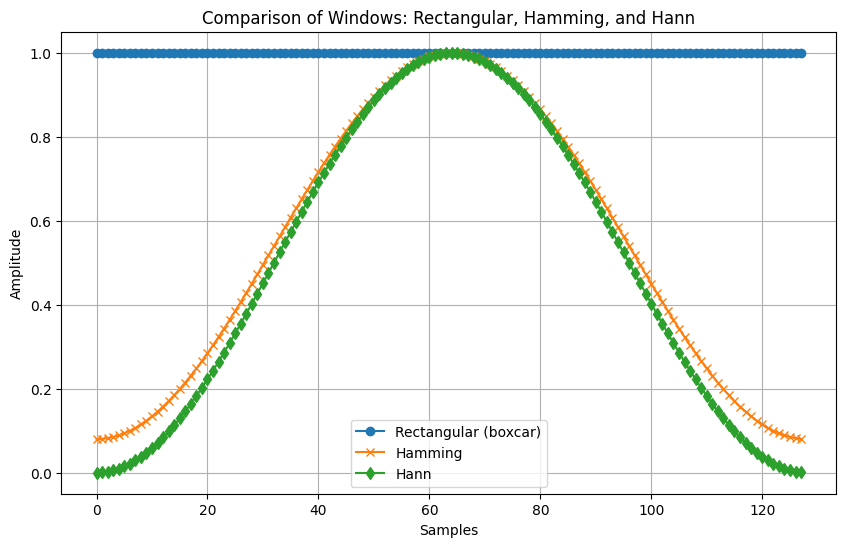
\includegraphics[width=0.7\textwidth]{./figures/Comparison of Windows.png}
	\caption{Comparison of Rectangular, Hamming, and Hann windows in the time domain.}
	\label{fig:time_domain}
\end{figure}

\newpage
	
\subsection*{Observations}
In the time domain, the three windows show distinct characteristics, summarized as follows:

\begin{itemize}
    \item \textbf{Rectangular Window:} The window maintains a constant amplitude of 1 across its entire length, which results in a sharp cut-off at the edges. This behavior leads to significant spectral leakage in the frequency domain.
    
    \item \textbf{Hamming Window:} The Hamming window tapers smoothly towards the edges, although it does not reach zero. This gradual tapering helps in reducing spectral leakage while maintaining relatively good frequency resolution.
    
    \item \textbf{Hann Window:} The Hann window also tapers smoothly, but unlike the Hamming window, it reaches an amplitude of zero at the edges. This smooth tapering to zero provides better suppression of leakage, though at the cost of wider main lobes in the frequency domain.
\end{itemize}


\subsection{Frequency-Domain Comparison of Windows}
The Fourier Transforms of the Rectangular, Hamming, and Hann windows are computed, and their magnitude spectra are shown below.

\textbf{Python Code:}
\begin{lstlisting}[language=Python]
# Zero padding for FFT
zero_pad = 10000

# Apply FFT with zero padding and avoid log10(0) by adding a small epsilon value
epsilon = 1e-10  # Small value to avoid log(0)
rectangular_fft = 10 * np.log10(2 / zero_pad * (np.abs(fftshift(fft(rectangular_window, zero_pad))) + epsilon))
hamming_fft = 10 * np.log10(2 / zero_pad * (np.abs(fftshift(fft(hamming_window, zero_pad))) + epsilon))
hann_fft = 10 * np.log10(2 / zero_pad * (np.abs(fftshift(fft(hann_window, zero_pad))) + epsilon))

# Generate the corresponding frequencies
freqs = fftshift(fftfreq(zero_pad))

# Plot the spectra
plt.figure(figsize=(10, 6))
plt.plot(freqs, rectangular_fft, label='Rectangular (boxcar)')
plt.plot(freqs, hamming_fft, label='Hamming')
plt.plot(freqs, hann_fft, label='Hann')

# Configure labels and legend
plt.title('Magnitude Spectrum of Windows: Rectangular, Hamming, and Hann')
plt.xlabel('Normalized Frequency')
plt.ylabel('Magnitude (dB)')
plt.legend()
plt.grid(True)
plt.xlim([-0.05, 0.05])  # Limit the X-axis to better view the main lobe
plt.show()
\end{lstlisting}
\begin{figure}[H]
	\centering
	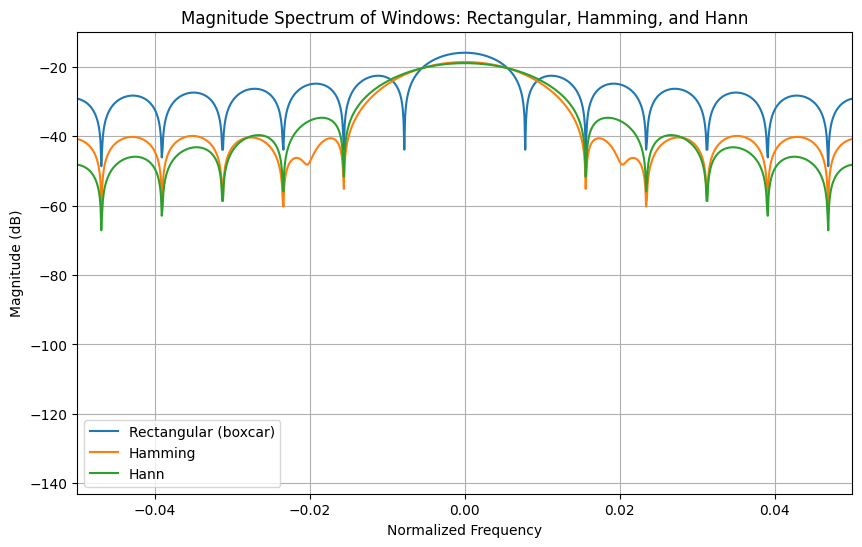
\includegraphics[width=0.6\textwidth]{./figures/Magnitude Spectrum of Windows.png}
	\caption{Magnitude spectrum of Rectangular, Hamming, and Hann windows.}
	\label{fig:freq_domain}
\end{figure}

\subsection*{Observations}
The analysis of the magnitude spectrum of the Rectangular, Hamming, and Hann windows leads to the following key observations:

\begin{itemize}
    \item \textbf{Rectangular Window:} This window exhibits the narrowest main lobe, which provides superior frequency resolution. However, it also presents the highest side lobes, causing significant spectral leakage. This makes it less suitable when side-lobe suppression is important.
    
    \item \textbf{Hamming Window:} The main lobe of the Hamming window is wider compared to the Rectangular window, which results in slightly lower frequency resolution. Nevertheless, the side lobes are considerably smaller, leading to reduced spectral leakage.
    
    \item \textbf{Hann Window:} Among the three, the Hann window has the widest main lobe, thus offering the lowest frequency resolution. However, its side lobes are the smallest, providing the best suppression of spectral leakage. This makes it particularly effective in applications where leakage minimization is prioritized.
\end{itemize}

\subsection{Discussion of Time-Domain and Frequency-Domain Representation}
The time-domain shape of a window has a direct influence on its behavior in the frequency domain:

\begin{itemize}
    \item A \textbf{sharp cutoff} in the time domain, as seen with the Rectangular window, results in a narrow main lobe but produces large side lobes in the frequency domain. This translates into higher spectral leakage.

    \item \textbf{Smoother transitions}, as observed with the Hamming and Hann windows, lead to significantly better suppression of the side lobes in the frequency domain. However, this improvement in leakage suppression comes at the cost of a wider main lobe, which reduces frequency resolution.
\end{itemize}

Thus, there is a clear trade-off between leakage suppression and frequency resolution. The Hann window provides the best side-lobe suppression, while the Rectangular window excels in frequency resolution. The Hamming window offers a balanced compromise between these two factors.

\subsection{Trade-offs in Window Selection}
When comparing the windows, the trade-off between frequency resolution and spectral leakage becomes evident:

\begin{itemize}
    \item The \textbf{Rectangular window} has the narrowest main lobe, giving it the best frequency resolution, but it also suffers from the worst spectral leakage due to high side lobes.
    
    \item The \textbf{Hamming window} offers a moderate compromise, with reduced spectral leakage at the expense of some frequency resolution. This balance makes it suitable for many practical signal processing tasks.
    
    \item The \textbf{Hann window}, with the widest main lobe, provides the best suppression of spectral leakage. However, the trade-off is that it offers the least frequency resolution. It is ideal for applications where leakage minimization is more important than precise frequency resolution.
\end{itemize}

In most practical applications, the \textbf{Hamming window} is often preferred as it strikes a good balance between frequency resolution and spectral leakage suppression, making it versatile for a variety of signal processing needs.

\section{Time-Domain Signal Visualization}

We start by visualizing both the resting and sleep signals in the time domain to observe their characteristics.

\begin{lstlisting}[language=Python]
	# Function to load a signal from a .txt file
	def load_signal_from_txt(filename, total_time=10):
		# Load the signal from the .txt file
		signal = np.loadtxt(filename, delimiter=';')[0, :]
		fs = np.round(len(signal)) / total_time
		# Return the loaded signal
		return signal, int(fs)

	reposo, fs_reposo = load_signal_from_txt('./reposo.txt')

	plt.figure(figsize=(10, 6))
	plt.plot(np.linspace(0, 10, 10 * fs_reposo), reposo, label=r'$\sigma = 1$')
	plt.title('Rest Signal in Time Domain')
	plt.xlabel('Time (s)')
	plt.ylabel('Amplitude')
	plt.legend()

	sueno, fs_sueno = load_signal_from_txt('./sueno.txt')

	plt.figure(figsize=(10, 6))
	plt.plot(np.linspace(0, 10, 10 * fs_sueno), sueno, label=r'$\sigma = 1$')
	plt.title('Sleep Signal in Time Domain')
	plt.xlabel('Time (s)')
	plt.ylabel('Amplitude')
	plt.legend()
	plt.show()
\end{lstlisting}


\textbf{Observations:}
\begin{itemize}
	\item The \textbf{resting signal} appears stable, with relatively constant heart rate.
	\item The \textbf{sleep signal} shows more variability in both frequency and amplitude, reflecting physiological changes during different sleep stages.
\end{itemize}
\subsection{Spectrograms with Different Window Types}

Now we compute and visualize the spectrograms using three window types: Rectangular, Hamming, and Hann. We use a window size of 256 samples and a 50\% overlap.

\begin{lstlisting}[language=Python]
from scipy import signal

# Define function to calculate and display the spectrogram
def plot_spectrogram(sig, fs, window_type='hann', window_size=256, overlapping=0.5, title=''):
    f, t, Sxx = signal.spectrogram(sig, fs, window=window_type, nperseg=window_size,
                                   noverlap=int(window_size * overlapping), scaling='spectrum')
    plt.figure(figsize=(12, 6))
    plt.pcolormesh(t, f, 10 * np.log10(Sxx), shading='gouraud')
    plt.colorbar(label='Power Spectral Density (dB)')
    plt.ylabel('Frequency (Hz)')
    plt.xlabel('Time (s)')
    plt.title(title)
    plt.show()

# Common parameters
window_size = 256
overlapping = 0.5

# List of windows
windows = ['boxcar', 'hamming', 'hann']
window_names = ['Rectangular', 'Hamming', 'Hann']

# Signal at rest
for window, name in zip(windows, window_names):
    plot_spectrogram(reposo, fs_reposo, window_type=window, window_size=window_size,
                     overlapping=overlapping, title=f'Spectrogram (Rest) - Window {name}')

# Signal during sleep
for window, name in zip(windows, window_names):
    plot_spectrogram(sueno, fs_sueno, window_type=window, window_size=window_size,
                     overlapping=overlapping, title=f'Spectrogram (Sleep) - Window {name}')
\end{lstlisting}

\textbf{Observations:}
- \textbf{Rectangular window}: Causes spectral leakage, resulting in a blurred frequency representation.
- \textbf{Hamming and Hann windows}: Provide better frequency resolution with less leakage, making the frequency components more distinct.

\section*{3. Effect of Different Overlaps with Hamming Window}

Next, we analyze the effect of different overlap percentages: 0\%, 50\%, and 75\%, while using the Hamming window and a window size of 256 samples.

\begin{lstlisting}[caption=Python code for analyzing different overlap percentages]
# List of overlap percentages
overlaps = [0.0, 0.5, 0.75]
overlap_percentages = ['0%', '50%', '75%']

# Signal at rest with different overlaps
for overlap, percentage in zip(overlaps, overlap_percentages):
    plot_spectrogram(reposo, fs_reposo, window_type='hamming', window_size=256,
                     overlapping=overlap, title=f'Spectrogram (Rest) - Overlap {percentage}')

# Signal during sleep with different overlaps
for overlap, percentage in zip(overlaps, overlap_percentages):
    plot_spectrogram(sueno, fs_sueno, window_type='hamming', window_size=256,
                     overlapping=overlap, title=f'Spectrogram (Sleep) - Overlap {percentage}')
\end{lstlisting}

\textbf{Observations:}
- As the overlap increases, the spectrogram becomes smoother, and rapid changes are more detectable.
- With no overlap, there are visible discontinuities in the spectrogram.

\section*{4. Effect of Window Size on Spectrogram Resolution}

We now compare the spectrograms using different window sizes: 128, 256, and 512 samples, with a 50\% overlap.

\begin{lstlisting}[caption=Python code for analyzing different window sizes]
# List of window sizes
window_sizes = [128, 256, 512]
window_size_labels = ['128 samples', '256 samples', '512 samples']

# Spectrograms with different window sizes
for size, label in zip(window_sizes, window_size_labels):
    plot_spectrogram(reposo, fs_reposo, window_type='hamming', window_size=size,
                     overlapping=0.5, title=f'Spectrogram (Rest) - Window Size {label}')
\end{lstlisting}

\textbf{Observations:}
- Smaller windows (128 samples) offer better time resolution but poorer frequency resolution.
- Larger windows (512 samples) provide better frequency resolution but lose temporal precision.

\section*{5. Best Combination of Parameters}

Based on the analysis, the optimal combination of parameters for both signals (rest and sleep) is:
- \textbf{Window type}: Hamming
- \textbf{Window size}: 256 samples
- \textbf{Overlap}: 75\%

This configuration provides a good balance between time and frequency resolution.

\begin{lstlisting}[caption=Python code for optimal spectrogram generation]
# Spectrogram of the signal at rest with optimal parameters
plot_spectrogram(reposo, fs_reposo, window_type='hamming', window_size=256,
                 overlapping=0.75, title='Optimal Spectrogram (Rest)')

# Spectrogram of the signal during sleep with optimal parameters
plot_spectrogram(sueno, fs_sueno, window_type='hamming', window_size=256,
                 overlapping=0.75, title='Optimal Spectrogram (Sleep)')
\end{lstlisting}

\section*{6. Analysis of Optimal Spectrograms}

\begin{figure}[h]
    \centering
    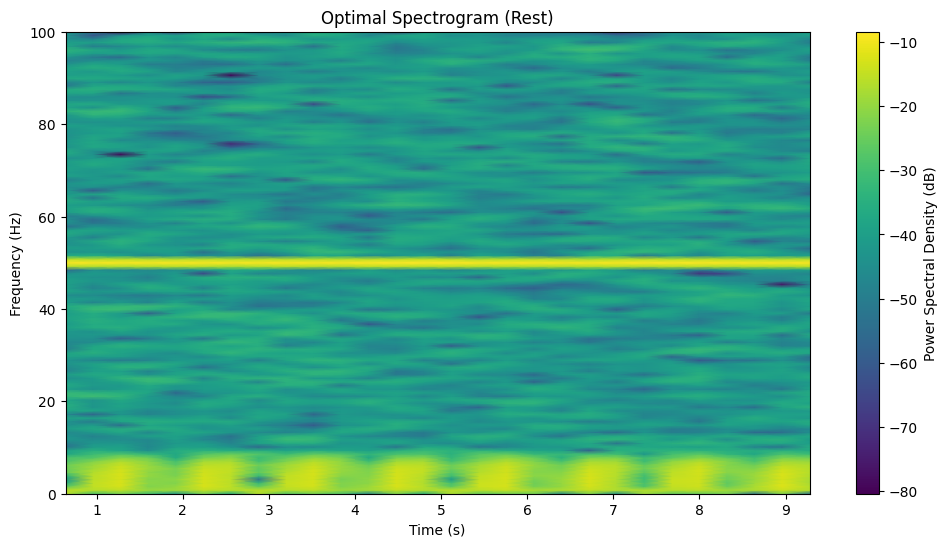
\includegraphics[width=0.8\textwidth]{./figures/Optimal Spectrogram (Rest).png}
    \caption{Optimal Spectrogram for Rest Signal}
\end{figure}

\begin{figure}[h]
    \centering
    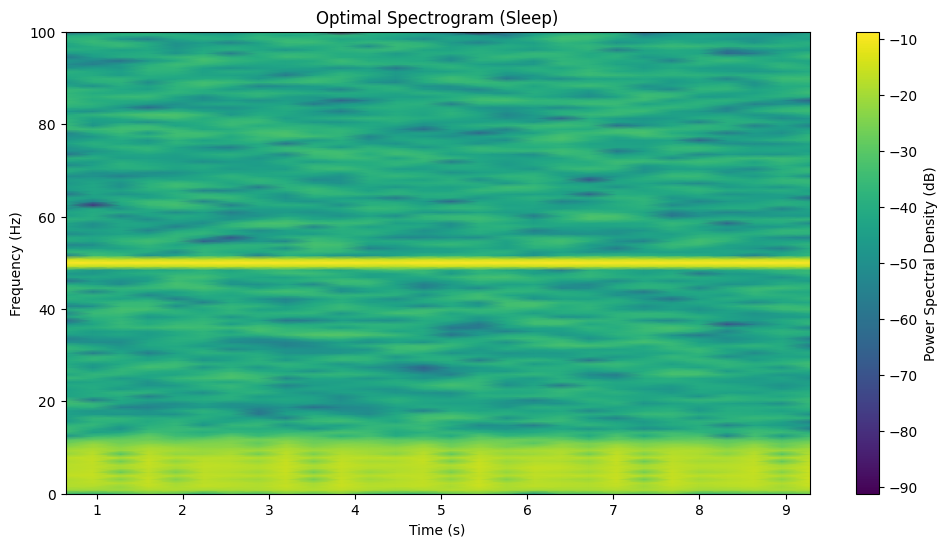
\includegraphics[width=0.8\textwidth]{./figures/Optimal Spectrogram (Sleep).png}
    \caption{Optimal Spectrogram for Sleep Signal}
\end{figure}

\textbf{Observations:}
- The resting signal exhibits a stable frequency, indicating regular heart rate.
- The sleep signal shows more variability, which may correspond to different sleep stages (e.g., REM and non-REM).

\textbf{Conclusion:} The use of spectrograms with appropriate parameter tuning provides significant insights into heart rate variability between rest and sleep, allowing for the detection of subtle physiological changes.

\end{document}


